\chapter{Resultados del estudio}

En este capítulo se recopilan las tablas y gráficas más representativas con los resultados obtenidos en el estudio. Se mostrará una tabla global para cada dimensión, que incluya el valor medio obtenido como solución por función y algoritmo, además de una tabla de rankings que ayude a determinar qué algoritmos se comportan mejor en general.

Además de las tablas, se incluirán algunas gráficas de convergencia para poder observar de manera más visual qué algoritmos llegan antes a los óptimos y cuáles necesitan de más evaluaciones, así como qué resultados son mejores y en qué proporción con respecto al resto.

Por último, se dará una visión analítica acerca de los resultados, dando pie a distintas valoraciones bien fundamentadas que se pueden extraer de las tablas para obtener las conclusiones del estudio.

\begin{table}
	\centering
	\resizebox{\textwidth}{!}{
	\begin{tabular}{cccccccc}
		\toprule
		{} &        \textbf{ASO} &         \textbf{IA} &        \textbf{ICA} &        \textbf{POA} &        \textbf{PSO} &        \textbf{SEA} &        \textbf{SLC} \\
		\midrule
		\textbf{F01}  &  5.071e+00 &  1.981e+03 &  6.705e+03 &  1.460e+04 &  2.828e+03 &  1.348e+01 &  \textbf{0.000e+00} \\
		\textbf{F02}  &  1.980e+02 &  3.436e+03 &  9.925e+03 &  1.297e+04 &  1.719e+04 &  1.292e+02 &  \textbf{1.160e-08} \\
		\textbf{F03}  &  1.137e+06 &  9.482e+06 &  5.012e+07 &  1.251e+08 &  9.043e+07 &  5.509e+06 &  \textbf{2.971e+04} \\
		\textbf{F04}  &  6.140e+01 &  4.165e+03 &  1.169e+04 &  1.365e+04 &  7.709e+04 &  9.347e+02 &  \textbf{3.592e-05} \\
		\textbf{F05}  &  8.036e+02 &  7.204e+03 &  8.684e+03 &  1.901e+04 &  1.752e+04 &  6.230e+02 &  \textbf{4.590e-03} \\
		\textbf{F06}  &  1.388e+04 &  6.219e+07 &  9.836e+08 &  3.383e+09 &  3.263e+08 &  2.764e+04 &  \textbf{8.802e+01} \\
		\textbf{F07}  &  5.061e+00 &  1.890e+03 &  1.259e+03 &  3.131e+03 &  2.253e+03 &  1.920e+03 &  \textbf{5.673e-01} \\
		\textbf{F08}  &  2.035e+01 &  2.041e+01 &  2.053e+01 &  2.093e+01 &  2.022e+01 &  2.028e+01 &  \textbf{2.019e+01} \\
		\textbf{F09}  &  \textbf{3.529e+00} &  6.505e+01 &  7.433e+01 &  8.867e+01 &  1.201e+02 &  3.292e+01 &  3.881e+00 \\
		\textbf{F10}  &  9.487e+00 &  9.127e+01 &  9.884e+01 &  1.162e+02 &  2.073e+02 &  2.739e+01 &  \textbf{4.584e+00} \\
		\textbf{F11}  &  7.778e+00 &  9.458e+00 &  1.028e+01 &  1.345e+01 &  7.542e+00 &  8.258e+00 &  \textbf{3.801e+00} \\
		\textbf{F12}  &  1.230e+03 &  2.248e+04 &  5.419e+04 &  1.107e+05 &  5.515e+04 &  2.686e+03 &  \textbf{4.385e+02} \\
		\textbf{F13}  &  \textbf{5.364e-01} &  6.426e+00 &  1.014e+01 &  9.040e+00 &  6.991e+00 &  2.393e+00 &  5.710e-01 \\
		\textbf{F14}  &  3.754e+00 &  3.927e+00 &  4.111e+00 &  4.501e+00 &  4.853e+00 &  3.606e+00 &  \textbf{2.460e+00} \\
		\textbf{F15}  &  \textbf{2.538e+02} &  5.274e+02 &  6.972e+02 &  9.631e+02 &  7.499e+02 &  4.281e+02 &  2.721e+02 \\
		\textbf{F16}  &  1.216e+02 &  2.799e+02 &  3.968e+02 &  6.118e+02 &  5.502e+02 &  1.679e+02 &  \textbf{1.108e+02} \\
		\textbf{F17}  &  5.554e+01 &  1.346e+02 &  8.380e+01 &  1.128e+02 &  2.099e+02 &  9.551e+01 &  \textbf{3.215e+01} \\
		\textbf{F18}  &  \textbf{7.774e+02} &  1.091e+03 &  1.129e+03 &  1.383e+03 &  1.245e+03 &  1.037e+03 &  8.838e+02 \\
		\textbf{F19}  &  \textbf{8.096e+02} &  1.084e+03 &  1.161e+03 &  1.383e+03 &  1.194e+03 &  8.563e+02 &  8.373e+02 \\
		\textbf{F20}  &  \textbf{8.158e+02} &  1.082e+03 &  1.161e+03 &  1.383e+03 &  1.267e+03 &  9.720e+02 &  8.648e+02 \\
		\textbf{F21}  &  7.045e+02 &  1.252e+03 &  1.340e+03 &  1.424e+03 &  1.384e+03 &  8.994e+02 &  \textbf{6.702e+02} \\
		\textbf{F22}  &  7.250e+02 &  9.516e+02 &  1.076e+03 &  1.350e+03 &  1.248e+03 &  8.940e+02 &  \textbf{6.624e+02} \\
		\textbf{F23}  &  9.590e+02 &  1.256e+03 &  1.317e+03 &  1.474e+03 &  1.391e+03 &  1.071e+03 &  \textbf{9.556e+02} \\
		\textbf{F24}  &  \textbf{2.365e+02} &  1.134e+03 &  1.164e+03 &  1.446e+03 &  1.459e+03 &  8.663e+02 &  2.800e+02 \\
		\textbf{F25}  &  \textbf{5.109e+02} &  1.346e+03 &  1.101e+03 &  2.118e+03 &  1.214e+03 &  5.243e+02 &  5.188e+02 \\
		\textbf{Best} &          8 &          0 &          0 &          0 &          0 &          0 &         \textbf{17} \\
		\bottomrule
\end{tabular}}
	\caption{Resultados medios del benchmark CEC2005 para dimensión 10.}
\end{table}

\begin{table}
	\centering
	\begin{tabular}{cccccccc}
		\toprule
		{} &    \textbf{ASO} &     \textbf{IA} &    \textbf{ICA} &    \textbf{POA} &    \textbf{PSO} &    \textbf{SEA} &    \textbf{SLC} \\
		\midrule
		\textbf{F01}  &      2 &      4 &      6 &      7 &      5 &      3 &      \textbf{1} \\
		\textbf{F02}  &      3 &      4 &      5 &      6 &      7 &      2 &      \textbf{1} \\
		\textbf{F03}  &      2 &      4 &      5 &      7 &      6 &      3 &      \textbf{1} \\
		\textbf{F04}  &      2 &      4 &      5 &      6 &      7 &      3 &      \textbf{1} \\
		\textbf{F05}  &      3 &      4 &      5 &      7 &      6 &      2 &      \textbf{1} \\
		\textbf{F06}  &      2 &      4 &      6 &      7 &      5 &      3 &      \textbf{1} \\
		\textbf{F07}  &      2 &      4 &      3 &      7 &      6 &      5 &      \textbf{1} \\
		\textbf{F08}  &      4 &      5 &      6 &      7 &      2 &      3 &      \textbf{1} \\
		\textbf{F09}  &      \textbf{1} &      4 &      5 &      6 &      7 &      3 &      2 \\
		\textbf{F10}  &      2 &      4 &      5 &      6 &      7 &      3 &      \textbf{1} \\
		\textbf{F11}  &      3 &      5 &      6 &      7 &      2 &      4 &      \textbf{1} \\
		\textbf{F12}  &      2 &      4 &      5 &      7 &      6 &      3 &      \textbf{1} \\
		\textbf{F13}  &      \textbf{1} &      4 &      7 &      6 &      5 &      3 &      2 \\
		\textbf{F14}  &      3 &      4 &      5 &      6 &      7 &      2 &      \textbf{1} \\
		\textbf{F15}  &      \textbf{1} &      4 &      5 &      7 &      6 &      3 &      2 \\
		\textbf{F16}  &      2 &      4 &      5 &      7 &      6 &      3 &      \textbf{1} \\
		\textbf{F17}  &      2 &      6 &      3 &      5 &      7 &      4 &      \textbf{1} \\
		\textbf{F18}  &      \textbf{1} &      4 &      5 &      7 &      6 &      3 &      2 \\
		\textbf{F19}  &      \textbf{1} &      4 &      5 &      7 &      6 &      3 &      2 \\
		\textbf{F20}  &      \textbf{1} &      4 &      5 &      7 &      6 &      3 &      2 \\
		\textbf{F21}  &      2 &      4 &      5 &      7 &      6 &      3 &      \textbf{1} \\
		\textbf{F22}  &      2 &      4 &      5 &      7 &      6 &      3 &      \textbf{1} \\
		\textbf{F23}  &      2 &      4 &      5 &      7 &      6 &      3 &      \textbf{1} \\
		\textbf{F24}  &      \textbf{1} &      4 &      5 &      6 &      7 &      3 &      2 \\
		\textbf{F25}  &      \textbf{1} &      6 &      4 &      7 &      5 &      3 &      2 \\
		\textbf{Mean} &  1.920 &  4.240 &  5.040 &  6.640 &  5.800 &  3.040 &  \textbf{1.320} \\
		\bottomrule
	\end{tabular}
	\caption{Ranking de resultados del benchmark CEC2005 para dimensión 10.}
\end{table}

\begin{table}
	\resizebox{\textwidth}{!}{
	\begin{tabular}{cccccccc}
		\toprule
		{} &        \textbf{ASO} &         \textbf{IA} &        \textbf{ICA} &        \textbf{POA} &        \textbf{PSO} &        \textbf{SEA} &        \textbf{SLC} \\
		\midrule
		\textbf{F01}  &  1.288e+02 &  3.626e+04 &  6.173e+04 &  6.584e+04 &  8.855e+04 &  1.866e+03 &  \textbf{0.000e+00} \\
		\textbf{F02}  &  2.489e+03 &  4.569e+04 &  7.734e+04 &  8.917e+04 &  1.313e+05 &  1.220e+04 &  \textbf{1.179e-02} \\
		\textbf{F03}  &  1.602e+07 &  3.321e+08 &  1.194e+09 &  1.466e+09 &  1.633e+09 &  2.487e+07 &  \textbf{5.643e+05} \\
		\textbf{F04}  &  1.092e+04 &  5.443e+04 &  1.054e+05 &  8.943e+04 &  5.277e+05 &  3.946e+04 &  \textbf{4.680e+00} \\
		\textbf{F05}  &  4.663e+03 &  2.588e+04 &  3.480e+04 &  4.441e+04 &  4.695e+04 &  1.343e+04 &  \textbf{4.157e+03} \\
		\textbf{F06}  &  1.317e+07 &  9.779e+09 &  3.827e+10 &  2.916e+10 &  6.250e+10 &  1.173e+08 &  \textbf{7.574e+02} \\
		\textbf{F07}  &  1.646e+02 &  8.951e+03 &  9.200e+03 &  1.252e+04 &  1.069e+04 &  5.696e+03 &  \textbf{3.926e-01} \\
		\textbf{F08}  &  2.097e+01 &  2.096e+01 &  2.112e+01 &  2.134e+01 &  \textbf{2.064e+01} &  2.082e+01 &  2.090e+01 \\
		\textbf{F09}  &  \textbf{2.940e+01} &  3.278e+02 &  4.076e+02 &  4.047e+02 &  4.455e+02 &  2.046e+02 &  9.910e+01 \\
		\textbf{F10}  &  2.528e+02 &  4.707e+02 &  6.905e+02 &  6.595e+02 &  9.259e+02 &  2.872e+02 &  \textbf{9.004e+01} \\
		\textbf{F11}  &  3.956e+01 &  4.008e+01 &  4.330e+01 &  4.749e+01 &  3.427e+01 &  3.429e+01 &  \textbf{2.410e+01} \\
		\textbf{F12}  &  2.710e+04 &  1.026e+06 &  1.512e+06 &  1.579e+06 &  4.473e+05 &  1.481e+05 &  \textbf{9.489e+03} \\
		\textbf{F13}  &  3.567e+00 &  8.211e+01 &  1.858e+02 &  4.855e+01 &  1.075e+02 &  1.657e+01 &  \textbf{3.425e+00} \\
		\textbf{F14}  &  1.352e+01 &  1.359e+01 &  1.381e+01 &  1.437e+01 &  1.488e+01 &  1.337e+01 &  \textbf{1.207e+01} \\
		\textbf{F15}  &  \textbf{2.950e+02} &  8.825e+02 &  1.049e+03 &  1.200e+03 &  9.587e+02 &  6.849e+02 &  5.160e+02 \\
		\textbf{F16}  &  \textbf{8.460e+01} &  6.003e+02 &  9.486e+02 &  1.191e+03 &  8.238e+02 &  4.667e+02 &  2.964e+02 \\
		\textbf{F17}  &  5.693e+01 &  1.875e+02 &  8.462e+01 &  1.054e+02 &  2.195e+02 &  1.872e+02 &  \textbf{1.831e+01} \\
		\textbf{F18}  &  9.354e+02 &  1.184e+03 &  1.284e+03 &  1.268e+03 &  1.402e+03 &  9.586e+02 &  \textbf{9.107e+02} \\
		\textbf{F19}  &  \textbf{9.170e+02} &  1.178e+03 &  1.283e+03 &  1.261e+03 &  1.367e+03 &  9.666e+02 &  9.192e+02 \\
		\textbf{F20}  &  9.170e+02 &  1.158e+03 &  1.283e+03 &  1.261e+03 &  1.365e+03 &  9.758e+02 &  \textbf{9.094e+02} \\
		\textbf{F21}  &  \textbf{6.006e+02} &  1.325e+03 &  1.412e+03 &  1.386e+03 &  1.419e+03 &  1.066e+03 &  7.375e+02 \\
		\textbf{F22}  &  9.227e+02 &  1.306e+03 &  1.558e+03 &  1.740e+03 &  1.599e+03 &  1.193e+03 &  \textbf{9.108e+02} \\
		\textbf{F23}  &  9.780e+02 &  1.323e+03 &  1.383e+03 &  1.385e+03 &  1.422e+03 &  1.211e+03 &  \textbf{9.097e+02} \\
		\textbf{F24}  &  \textbf{2.021e+02} &  1.367e+03 &  1.468e+03 &  1.464e+03 &  1.602e+03 &  1.220e+03 &  9.086e+02 \\
		\textbf{F25}  &  \textbf{3.574e+02} &  1.410e+03 &  1.746e+03 &  1.978e+03 &  1.563e+03 &  9.508e+02 &  3.995e+02 \\
		\textbf{Best} &          7 &          0 &          0 &          0 &          1 &          0 &         \textbf{17} \\
		\bottomrule
\end{tabular}}
	\caption{Resultados medios del benchmark CEC2005 para dimensión 30.}
\end{table}

\begin{table}
	\centering
	\begin{tabular}{cccccccc}
		\toprule
		{} &    \textbf{ASO} &     \textbf{IA} &    \textbf{ICA} &    \textbf{POA} &    \textbf{PSO} &    \textbf{SEA} &    \textbf{SLC} \\
		\midrule
		\textbf{F01}  &      2 &      4 &      5 &      6 &      7 &      3 &      \textbf{1} \\
		\textbf{F02}  &      2 &      4 &      5 &      6 &      7 &      3 &      \textbf{1} \\
		\textbf{F03}  &      2 &      4 &      5 &      6 &      7 &      3 &      \textbf{1} \\
		\textbf{F04}  &      2 &      4 &      6 &      5 &      7 &      3 &      \textbf{1} \\
		\textbf{F05}  &      2 &      4 &      5 &      6 &      7 &      3 &      \textbf{1} \\
		\textbf{F06}  &      2 &      4 &      6 &      5 &      7 &      3 &      \textbf{1} \\
		\textbf{F07}  &      2 &      4 &      5 &      7 &      6 &      3 &      \textbf{1} \\
		\textbf{F08}  &      5 &      4 &      6 &      7 &      \textbf{1} &      2 &      3 \\
		\textbf{F09}  &      \textbf{1} &      4 &      6 &      5 &      7 &      3 &      2 \\
		\textbf{F10}  &      2 &      4 &      6 &      5 &      7 &      3 &      \textbf{1} \\
		\textbf{F11}  &      4 &      5 &      6 &      7 &      2 &      3 &      \textbf{1} \\
		\textbf{F12}  &      2 &      5 &      6 &      7 &      4 &      3 &      \textbf{1} \\
		\textbf{F13}  &      2 &      5 &      7 &      4 &      6 &      3 &      \textbf{1} \\
		\textbf{F14}  &      3 &      4 &      5 &      6 &      7 &      2 &      \textbf{1} \\
		\textbf{F15}  &      \textbf{1} &      4 &      6 &      7 &      5 &      3 &      2 \\
		\textbf{F16}  &      \textbf{1} &      4 &      6 &      7 &      5 &      3 &      2 \\
		\textbf{F17}  &      2 &      6 &      3 &      4 &      7 &      5 &      \textbf{1} \\
		\textbf{F18}  &      2 &      4 &      6 &      5 &      7 &      3 &      \textbf{1} \\
		\textbf{F19}  &      \textbf{1} &      4 &      6 &      5 &      7 &      3 &      2 \\
		\textbf{F20}  &      2 &      4 &      6 &      5 &      7 &      3 &      \textbf{1} \\
		\textbf{F21}  &      \textbf{1} &      4 &      6 &      5 &      7 &      3 &      2 \\
		\textbf{F22}  &      2 &      4 &      5 &      7 &      6 &      3 &      \textbf{1} \\
		\textbf{F23}  &      2 &      4 &      5 &      6 &      7 &      3 &      \textbf{1} \\
		\textbf{F24}  &      \textbf{1} &      4 &      6 &      5 &      7 &      3 &      2 \\
		\textbf{F25}  &      \textbf{1} &      4 &      6 &      7 &      5 &      3 &      2 \\
		\textbf{Mean} &  1.960 &  4.200 &  5.600 &  5.800 &  6.080 &  3.000 &  \textbf{1.360} \\
		\bottomrule
	\end{tabular}
	\caption{Ranking de resultados del benchmark CEC2005 para dimensión 30.}
\end{table}

\begin{table}
	\centering
	\begin{tabular}{lrr}
		\toprule
		{} &  \textbf{D-10} &  \textbf{D-30} \\
		\midrule
		\textbf{ASO} &   8 &   7 \\
		\textbf{IA}  &   0 &   0 \\
		\textbf{ICA} &   0 &   0 \\
		\textbf{POA} &   0 &   0 \\
		\textbf{PSO} &   0 &   1 \\
		\textbf{SEA} &   0 &   0 \\
		\textbf{SLC} &  \textbf{17} &  \textbf{17} \\
		\bottomrule
	\end{tabular}
	\caption{Mejores soluciones de cada algoritmo para cada dimensión.}
\end{table}

\begin{table}
	\centering
	\begin{tabular}{lrr}
		\toprule
		{} &    \textbf{D-10} &    \textbf{D-30} \\
		\midrule
		\textbf{ASO} &  1.92 &  1.96 \\
		\textbf{IA}  &  4.24 &  4.20 \\
		\textbf{ICA} &  5.04 &  5.60 \\
		\textbf{POA} &  6.64 &  5.80 \\
		\textbf{PSO} &  5.80 &  6.08 \\
		\textbf{SEA} &  3.04 &  3.00 \\
		\textbf{SLC} &  \textbf{1.32} &  \textbf{1.36} \\
		\bottomrule
	\end{tabular}
	\caption{Ranking global de cada algoritmo para cada dimensión.}
\end{table}

\begin{figure}
	\centering
	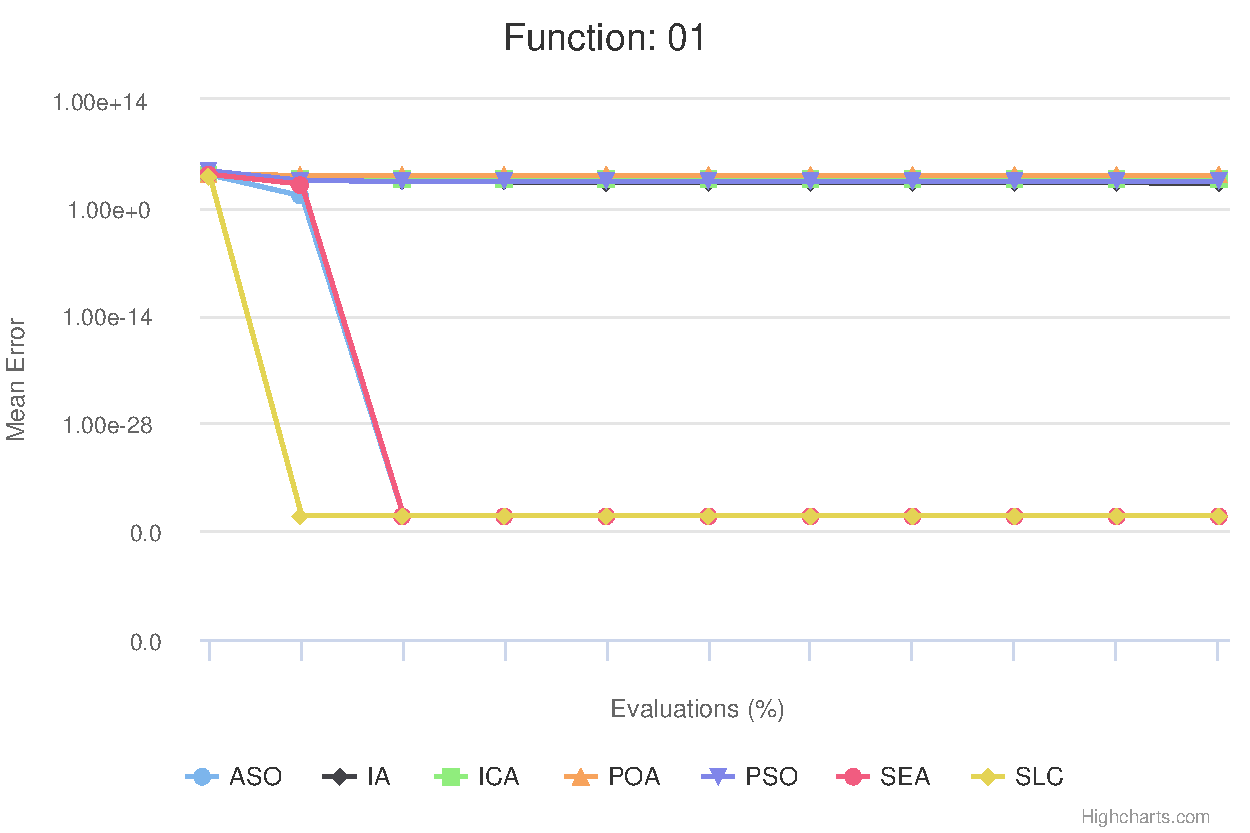
\includegraphics[scale=0.6]{imagenes/grafica-convergencia-1.pdf}
	\caption{Gráfica de convergencia de la función 1 para dimensión 10.}
	\label{grafica-convergencia-1}
\end{figure}

\begin{figure}
	\centering
	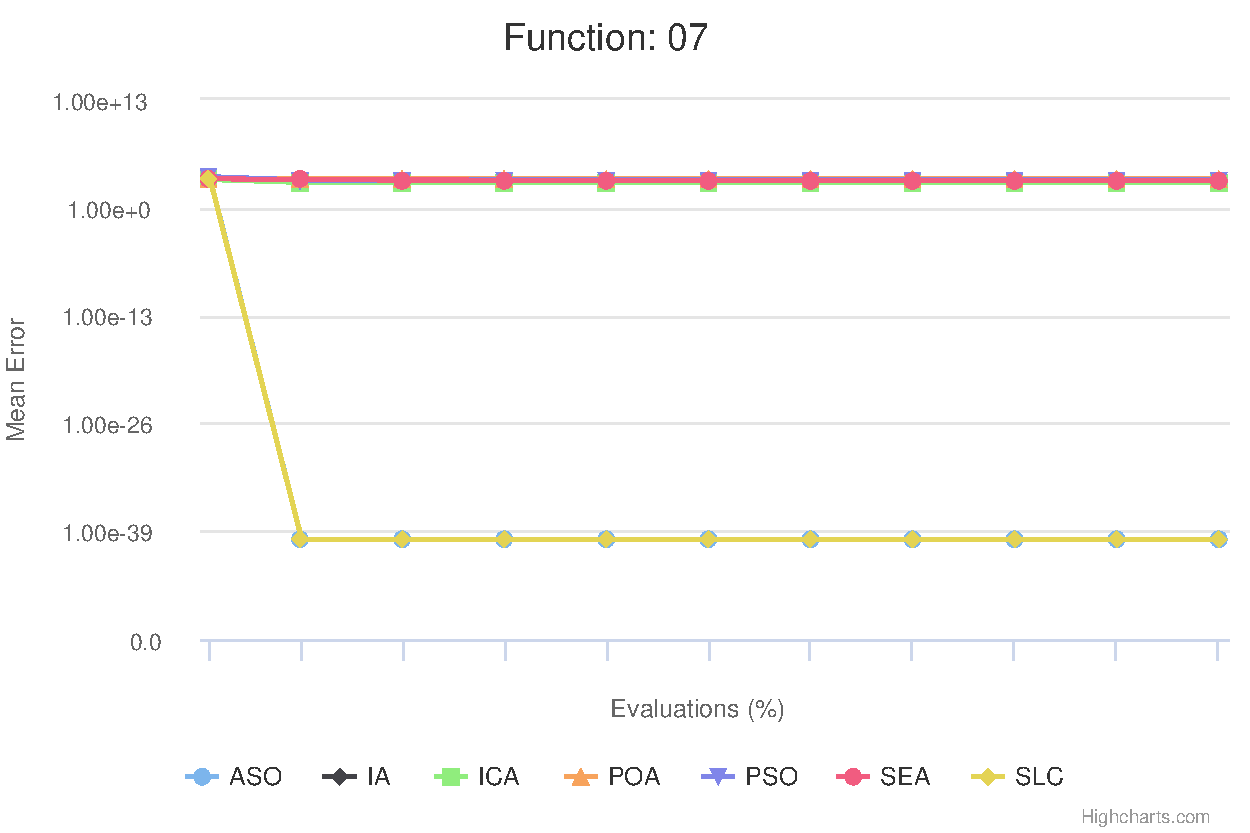
\includegraphics[scale=0.6]{imagenes/grafica-convergencia-7.pdf}
	\caption{Gráfica de convergencia de la función 7 para dimensión 10.}
	\label{grafica-convergencia-7}
\end{figure}

\begin{figure}
	\centering
	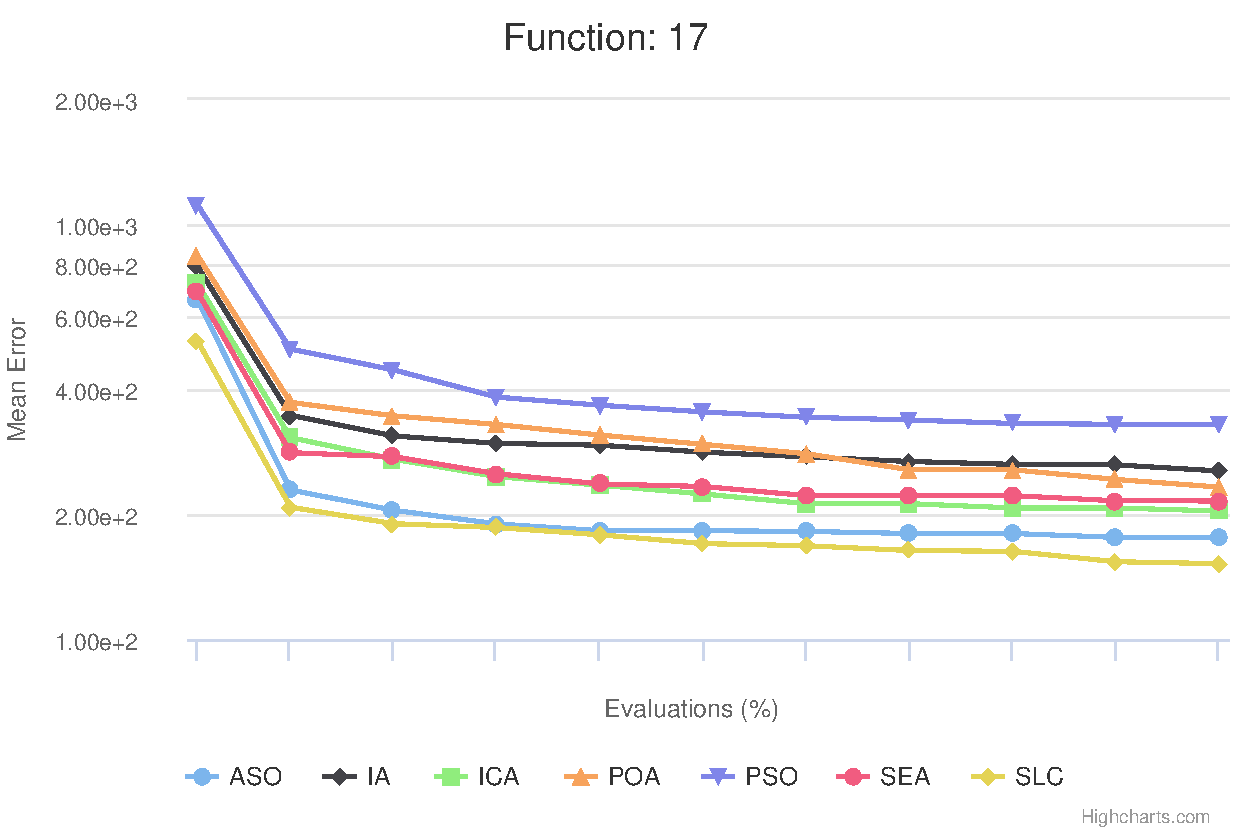
\includegraphics[scale=0.6]{imagenes/grafica-convergencia-17.pdf}
	\caption{Gráfica de convergencia de la función 17 para dimensión 10.}
	\label{grafica-convergencia-17}
\end{figure}